\section*{Appendix A}
Backfill  area increase in square kilometers in the study area. For both downsampled-, and full training data (TD).
\begin{table}[ht]
\centering
\caption{Backfill area increase per year [km$^2$] in the study area around Antananarivo. all TD = using all training data, ds TD = using downsampled training data.} 
\begin{tabular}{ccc}
  \hline
Backfill increase & Year & training data \\ 
  \hline
0.61 & 2014.00 & all TD \\ 
  0.72 & 2015.00 & all TD \\ 
  0.16 & 2016.00 & all TD \\ 
  1.54 & 2017.00 & all TD \\ 
  0.55 & 2018.00 & all TD \\ 
  0.75 & 2019.00 & all TD \\ 
  0.64 & 2020.00 & all TD \\ 
  0.30 & 2021.00 & all TD \\ 
  0.88 & 2022.00 & all TD \\ 
  0.80 & 2014.00 & ds TD \\ 
  0.68 & 2015.00 & ds TD \\ 
  0.18 & 2016.00 & ds TD \\ 
  1.81 & 2017.00 & ds TD \\ 
  0.59 & 2018.00 & ds TD \\ 
  0.83 & 2019.00 & ds TD \\ 
  0.72 & 2020.00 & ds TD \\ 
  0.27 & 2021.00 & ds TD \\ 
  0.93 & 2022.00 & ds TD \\ 
   \hline
\end{tabular}

\end{table}

\section*{Appendix B, pp. 39 - 45}
Classified maps resulting from the supervised classification
\section*{Appendix C, pp. 46 - 47}
Maps of backfill area increase per year between 2013 and 2022 in Antananarivo.


\begin{figure}[H]
    \centering
    \includegraphics[width = 15cm]{figures/classi2013.png}
    \caption{Classified image resulting from the 2013 classification.}
    \label{}
\end{figure}

\begin{figure}[H]
    \centering
    \includegraphics[width = 15cm]{figures/classi2014.png}
    \caption{Classified image resulting from the 2014 classification.}
    \label{}
\end{figure}

\begin{figure}[H]
    \centering
    \includegraphics[width = 15cm]{figures/classi2015.png}
    \caption{Classified image resulting from the 2015 classification.}
    \label{}
\end{figure}

\begin{figure}[H]
    \centering
    \includegraphics[width = 15cm]{figures/classi2018.png}
    \caption{Classified image resulting from the 2018 classification.}
    \label{}
\end{figure}

\begin{figure}[H]
    \centering
    \includegraphics[width = 15cm]{figures/classi2019.png}
    \caption{Classified image resulting from the 2019 classification.}
    \label{}
\end{figure}

\begin{figure}[H]
    \centering
    \includegraphics[width = 15cm]{figures/classi2020.png}
    \caption{Classified image resulting from the 2020 classification.}
    \label{}
\end{figure}

\begin{figure}[H]
    \centering
    \includegraphics[width = 15cm]{figures/classi2021.png}
    \caption{Classified image resulting from the 2021 classification.}
    \label{}
\end{figure}






\begin{rotatepage}
\begin{landscape}
\begin{figure}[H]
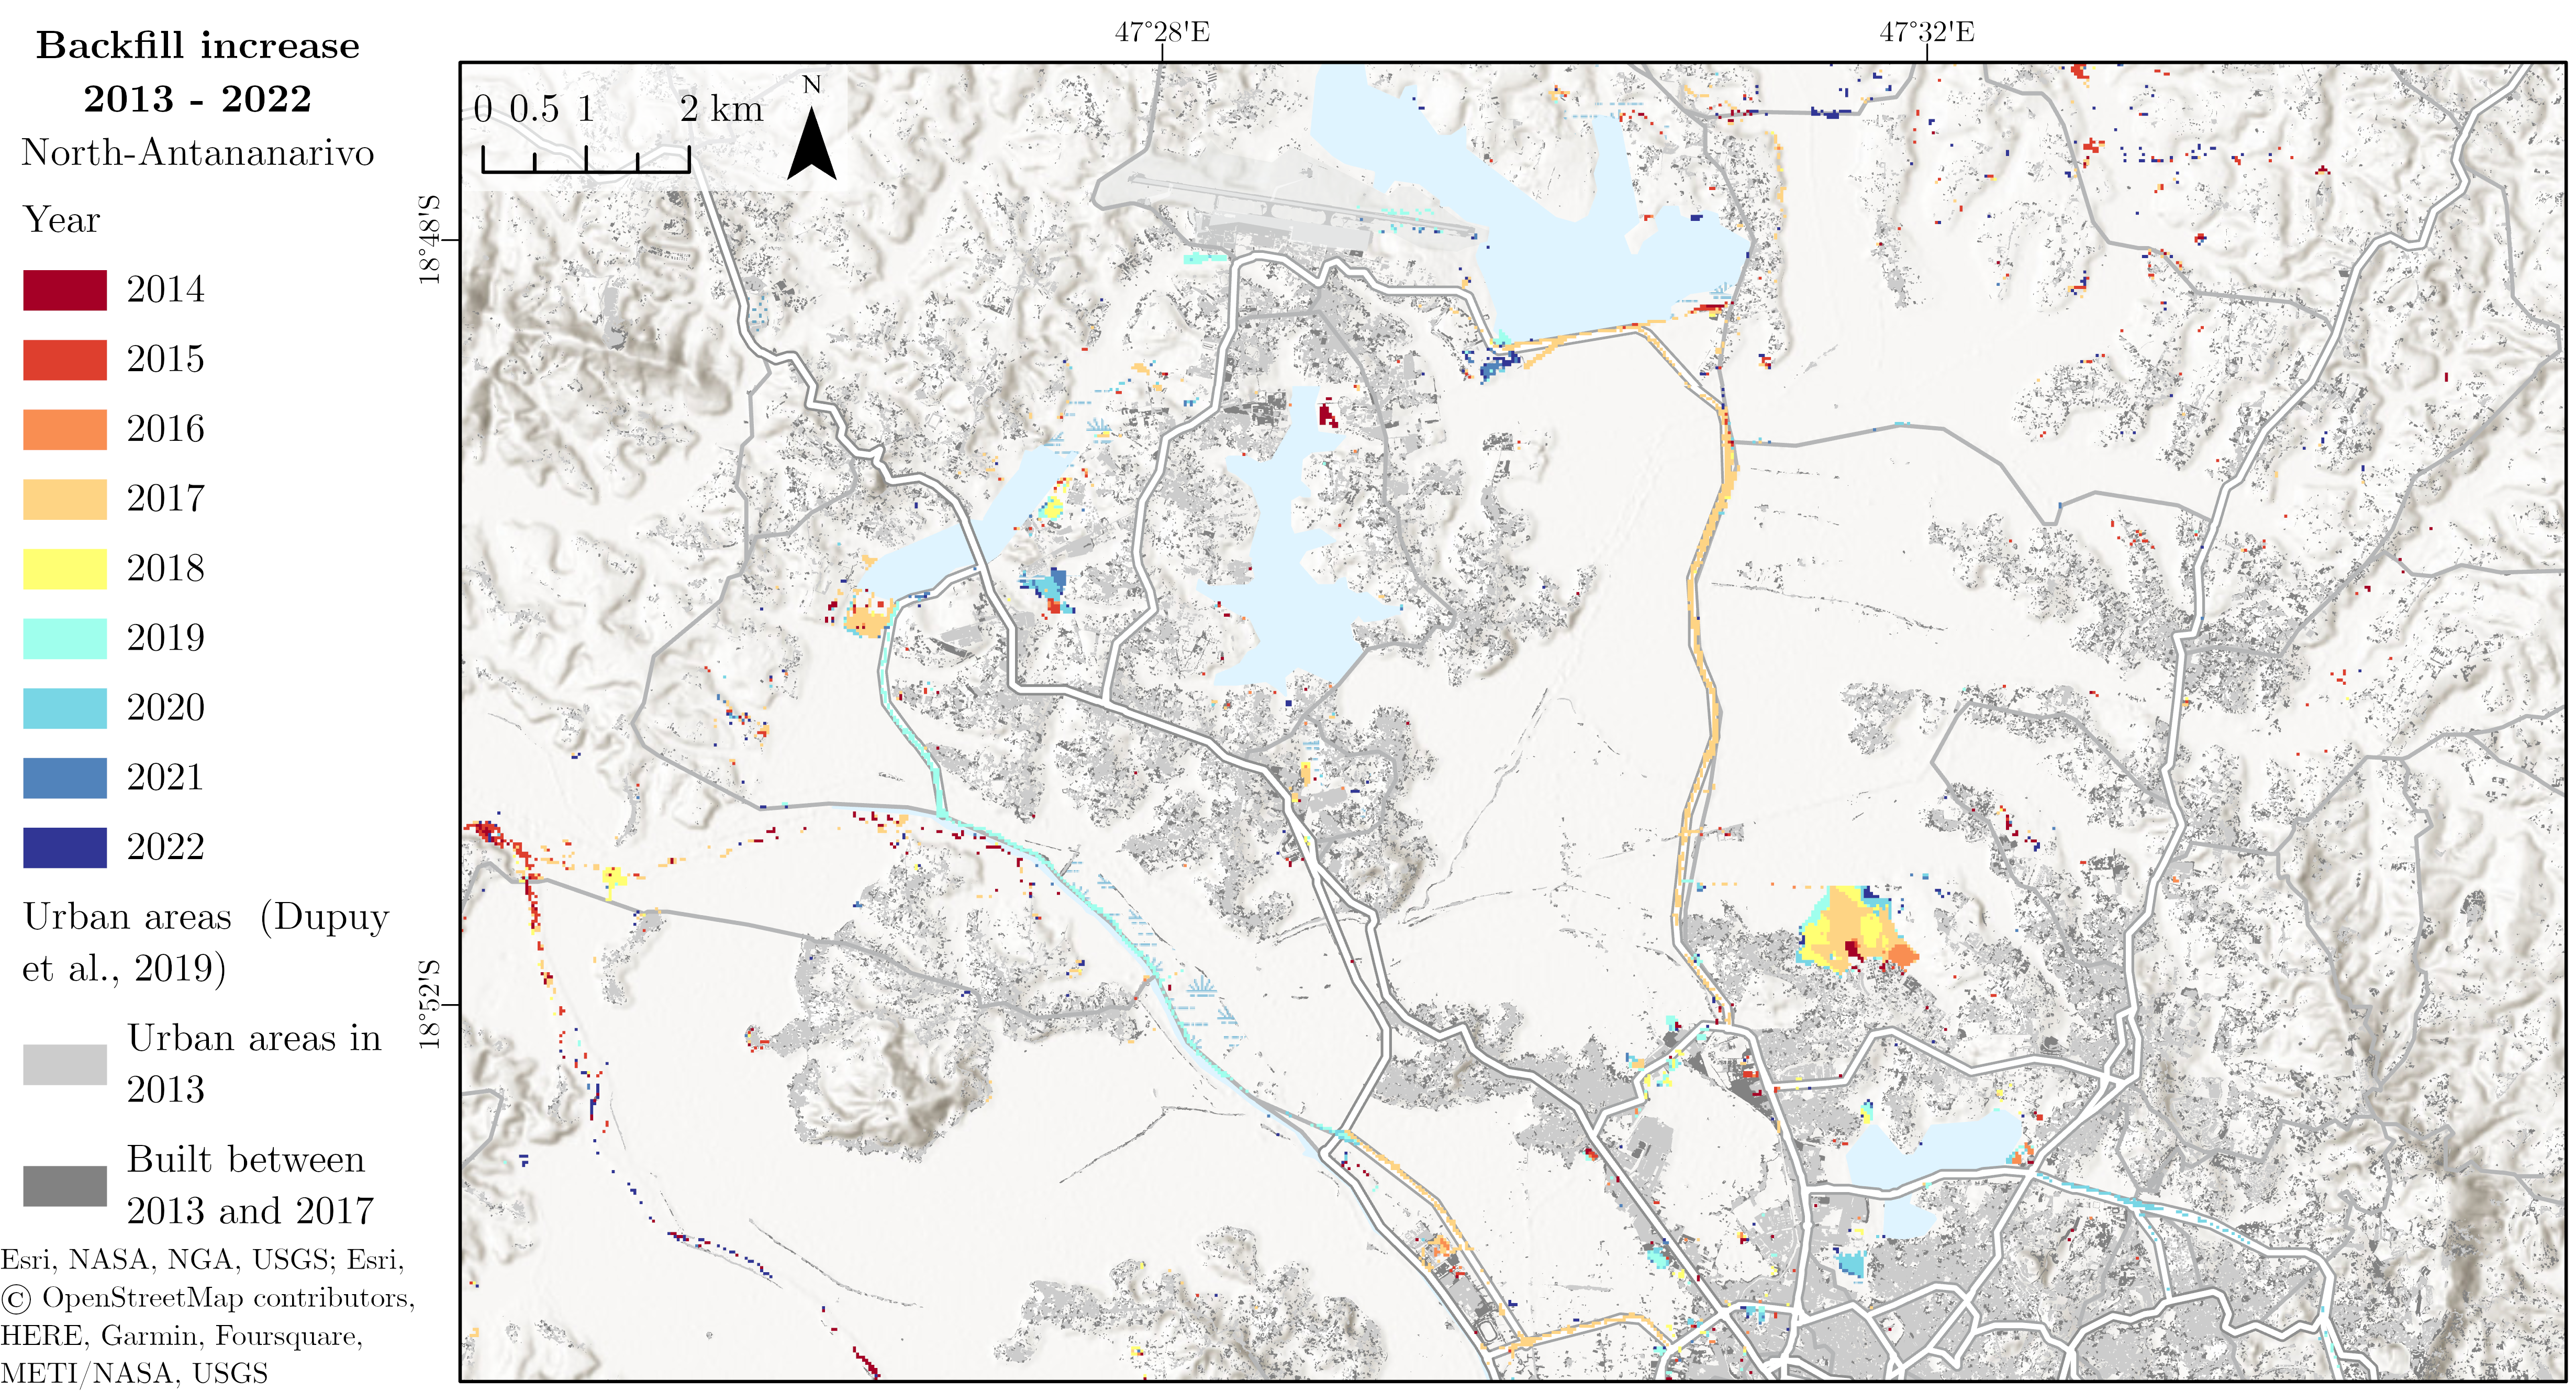
\includegraphics[width = 25cm]{figures/north_tana.png}
\caption{Backfill area increase per year in northern Antananarivo. The data showing urban ares in the map is sourced from \citet{Dupuy.2019}.}
\label{}
\end{figure}
\end{landscape}
\end{rotatepage}


\begin{rotatepage}
\begin{landscape}
\begin{figure}[H]
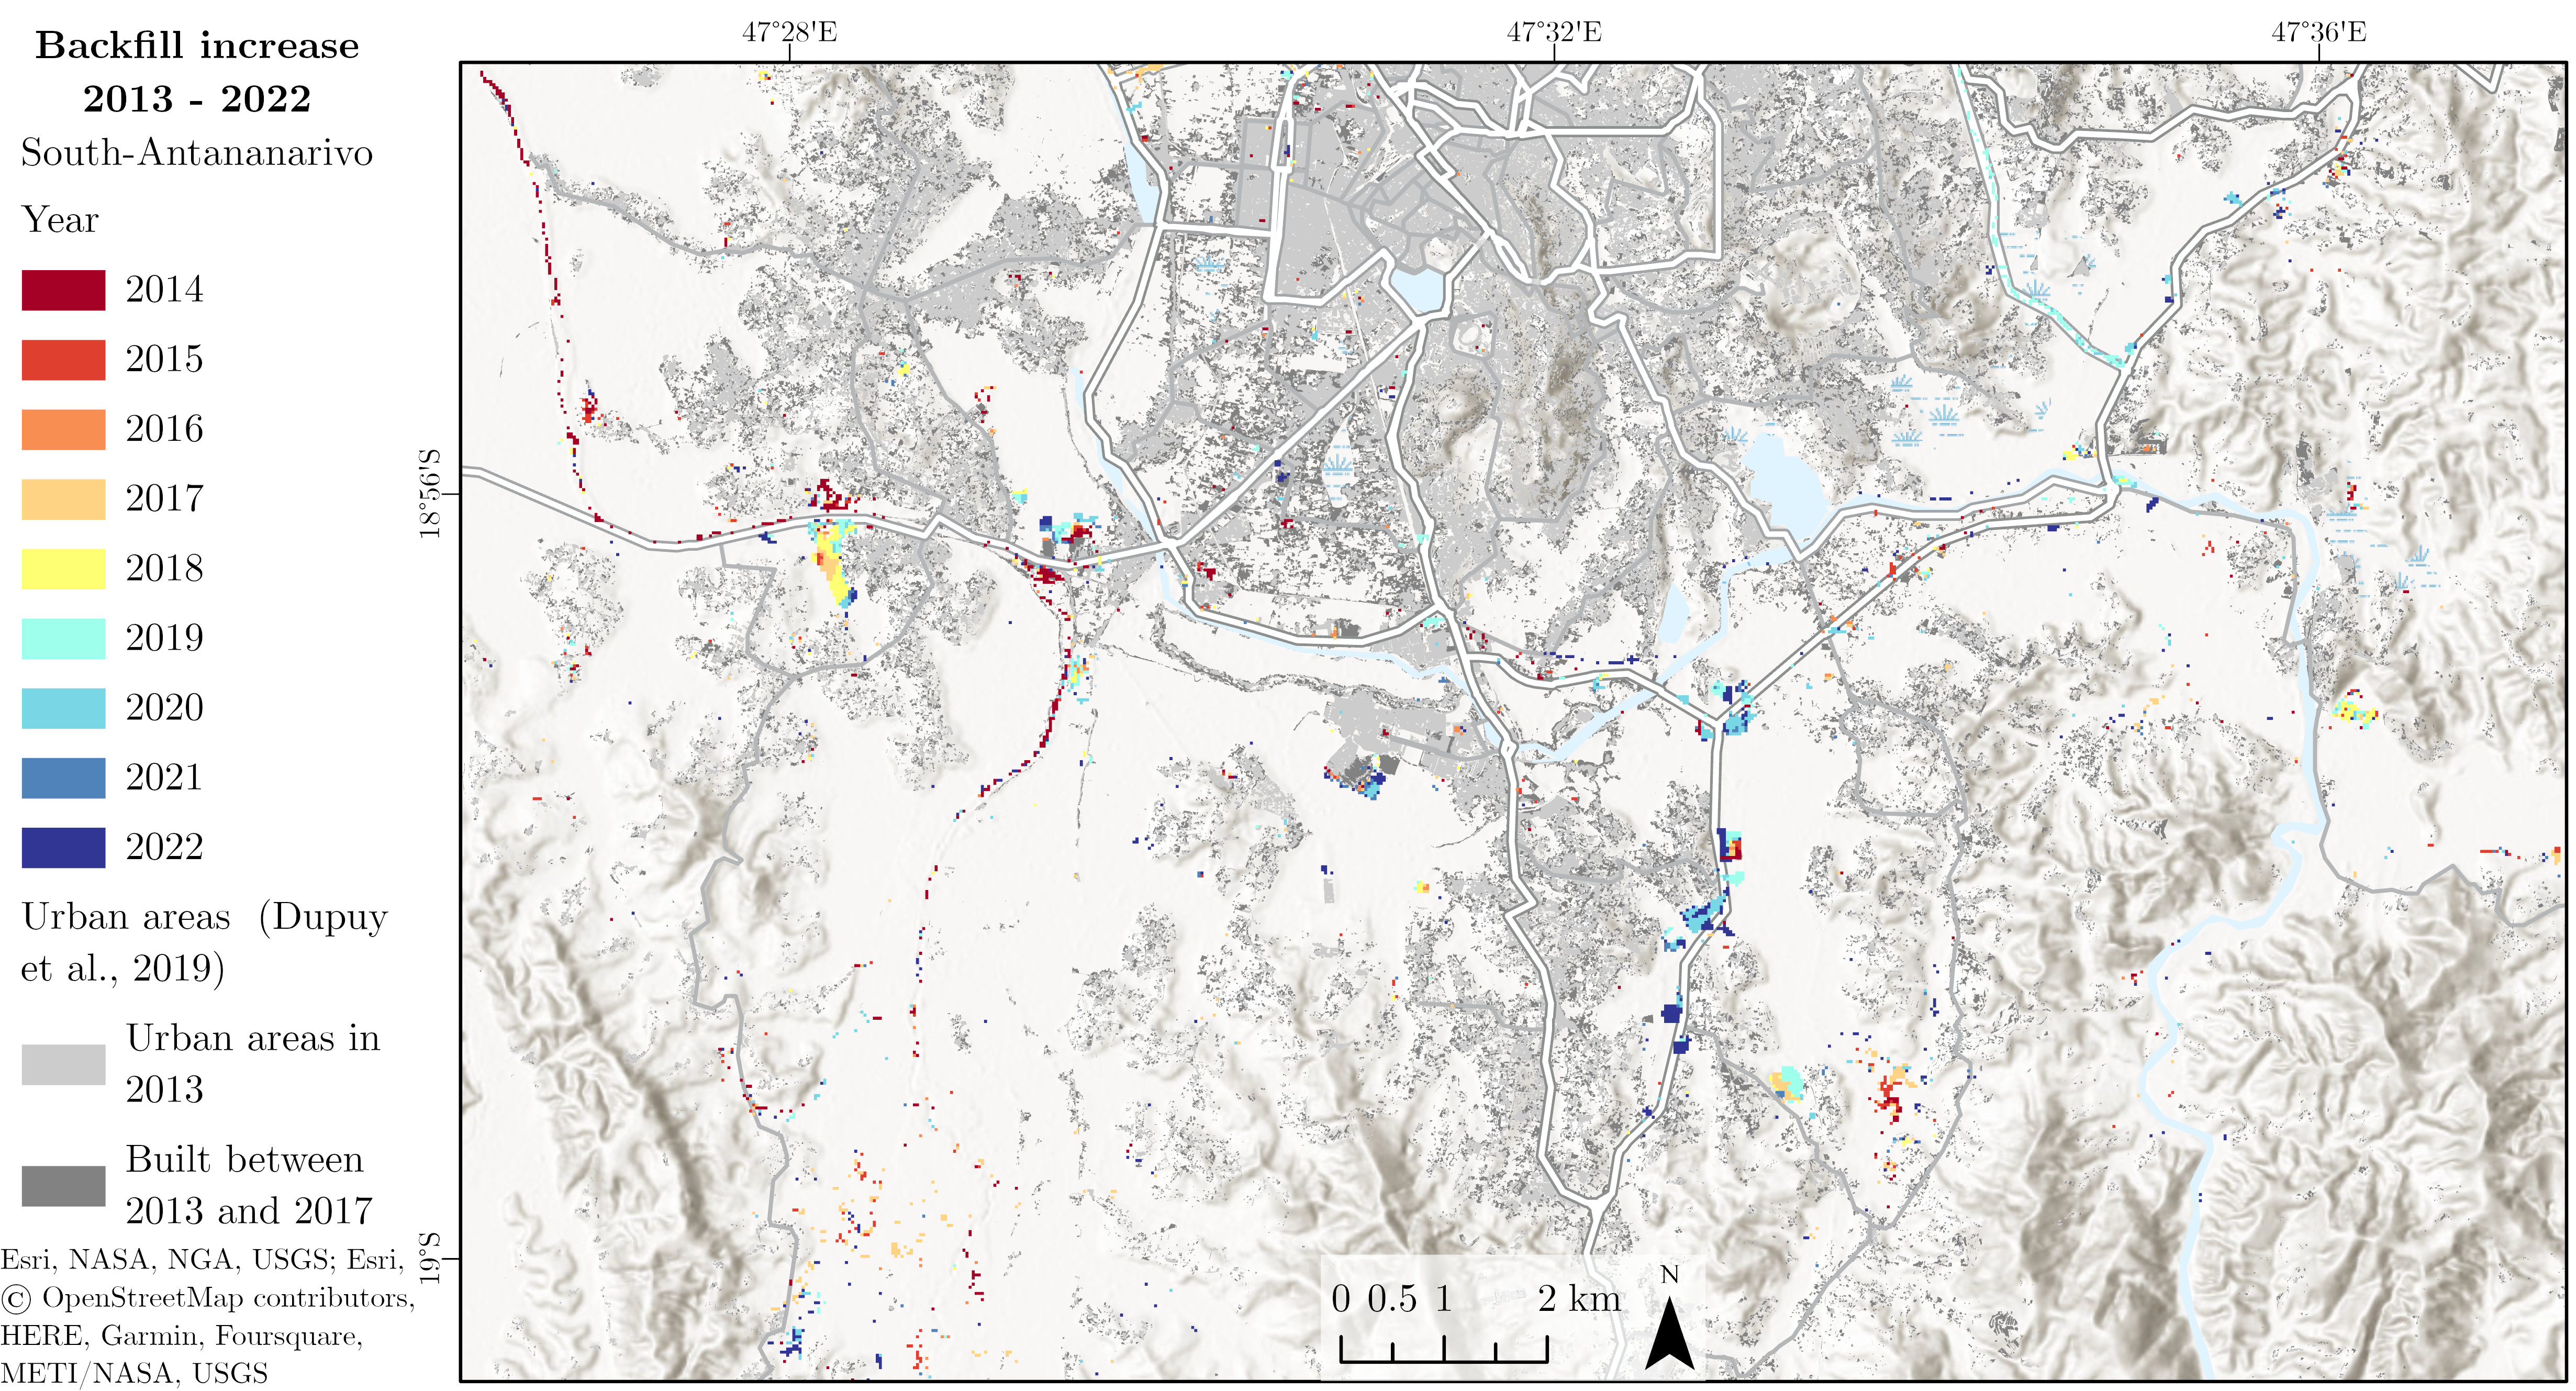
\includegraphics[width = 25cm]{figures/South_Tana.png}
\caption{Backfill area increase per year in southern Antananarivo. The data showing urban ares in the map is sourced from \citet{Dupuy.2019}.}
\label{}
\end{figure}
\end{landscape}
\end{rotatepage}